\chapter{Pixel Masking}\label{pixel_masking}

When analyzing diffraction data, not all of the pixels in 
an image should be used in the analysis. In order to make 
the program ignore certain pixels, 
this program allows for two types of pixel masking:
threshold masking and polygon masking. You can 
apply either of these from the 
\gui{Masking} tab shown in  figure~\ref{masking_tab}.

\section{Threshold Masking}

\begin{SCfigure}[1][bthp]
    \centering
    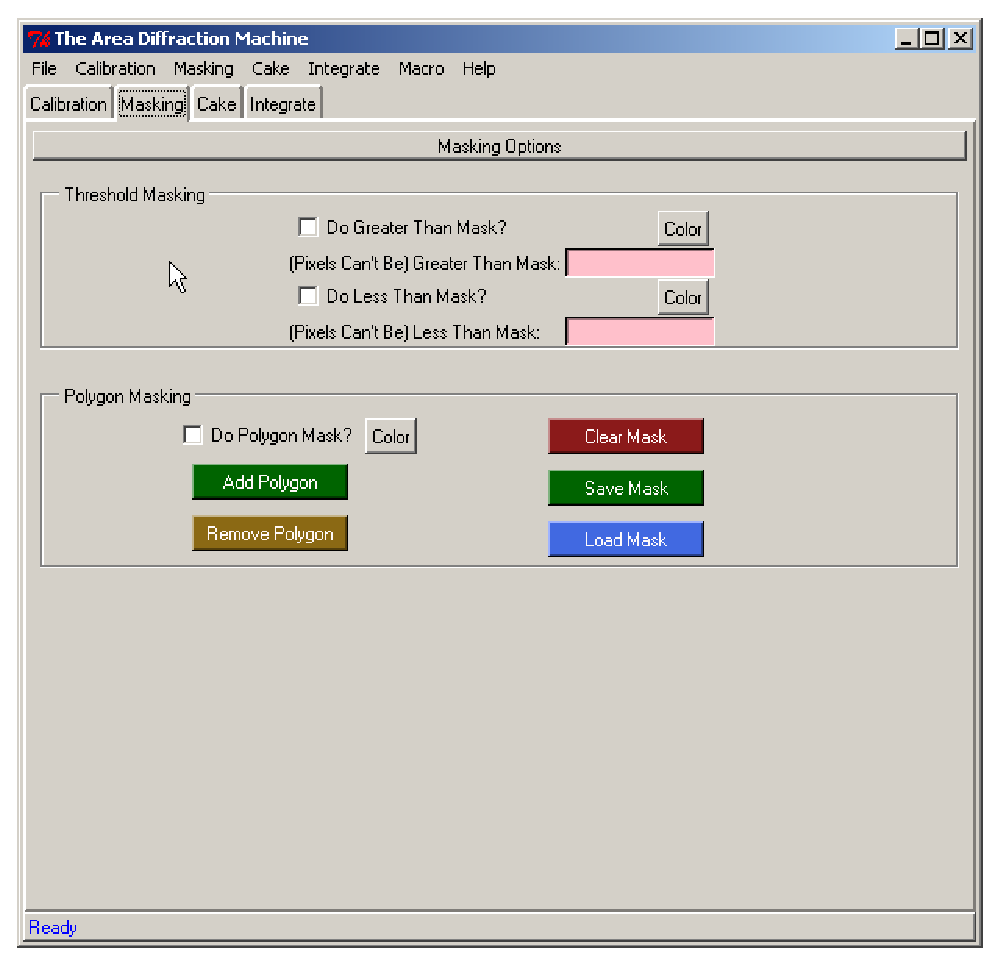
\includegraphics[scale=.75]{figures/masking_tab.eps}
    \caption{The pixel masking tab can be used to add
    a threshold mask or a polygon masking.} 
    \label{masking_tab}
\end{SCfigure}

The top half of the \gui{Masking} tab is devoted to 
threshold masking. Threshold masks allows all pixels, 
either above a certain intensity or below a certain 
intensity, to be ignored when doing the diffraction 
analysis. The \gui{Do Greater Than Mask?} check box can 
be used to apply a mask that will cause all pixels 
greater than a certain value to be ignored.
The \gui{(Pixel's Can't Be) Greater Than Mask} input 
can be used to specify the maximum pixel value.
The \gui{Do Less Than Mask} check box
can be used to make the program ignore all
pixels below a certain value. The particular value can 
be specified with the \gui{Less Than Mask} input. 

\begin{SCfigure}[1][bthp]
    \centering
    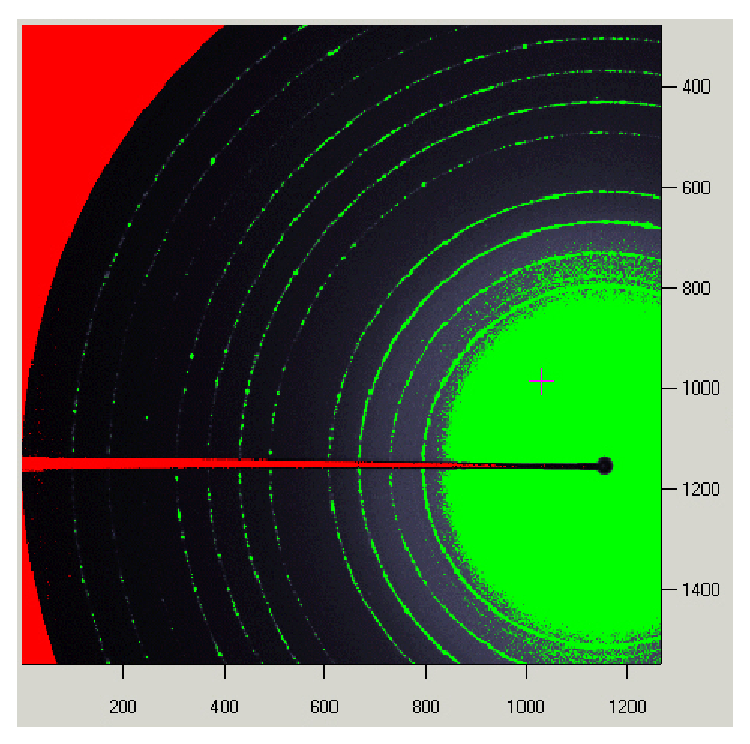
\includegraphics[scale=.75]{figures/Threshold_Masking.eps}
    \caption{A diffraction image with a
    greater than mask and less than mask.
    All pixels with intensity greater than 5000 
    have been colored green and all pixels with 
    intensity less than 30 have been colored red. Applying
    an intensity mask can be used to see if a detector's
    pixels have been overloaded. They can also be a used to
    ensure that overloaded pixels are not used in the
    data analysis.}
    \label{Threshold_Masking}
\end{SCfigure}

When applying a threshold mask, the pixels above or below
the threshold 
will be colored on the diffraction and cake image. 
The color can be set with the \gui{Color} button next to the greater 
than and less than masks. Figure~\ref{Threshold_Masking} shows 
diffraction image when all pixels
with intensity above 5000 are colored green and all pixels 
below 30 are colored red.

When caked data is saved, any of the pixels 
that are larger than the greater than mask are saved 
as -2. Any of the pixels smaller than the less than mask
are saved as -3. This behaviour needs to be accounted for
when analyzing caked data outside the program.

When an integrating intensity, 
any of the too high or too low pixels are simply ignored when 
calculating average intensity. 

\section{Polygon Masking}

Sometimes, large areas of a diffraction image should not
be included in the data analysis. For example, 
often a beam stop blocks part of the detector
and the pixels behind the beam stop should be ignored. 
This can be done with a polygon masks. Polygons can be drawn 
on the diffraction image and those parts 
of the image will not be used in subsequent analysis. 
This program can handle multiple polygons at the same time.

\begin{SCfigure}[1][bthp]
    \centering
    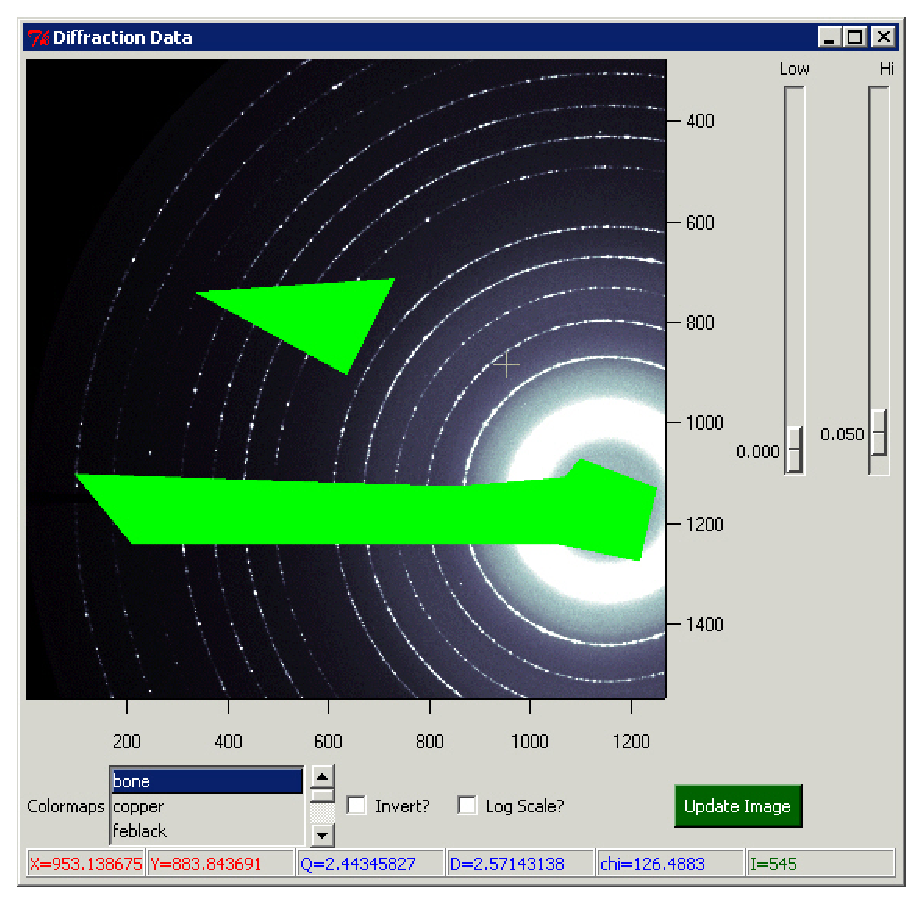
\includegraphics[scale=.75]{figures/Displayed_Polygon.eps}
    \caption{Two polygon masks that have been applied
    to this diffraction image. One of them covers the beam stop.}
    \label{Displayed_Polygon}
\end{SCfigure}

So long as the \gui{Do Polygon Mask?} check box is
selected, the polygon masks will be used 
when performing subsequent analysis. 
As figure~\ref{Displayed_Polygon} shows,
the polygons will be colored on the diffraction and
cake image.  The color of the polygon masks can be set 
with the \gui{Color} button
next to the \gui{Do Polygon Mask?} check box.
When caked data is saved, any pixels inside 
polygon masks will be given an intensity 
value of -4. During an intensity integration 
masked pixels will be ignored.

\begin{SCfigure}[1][bthp]
    \centering
    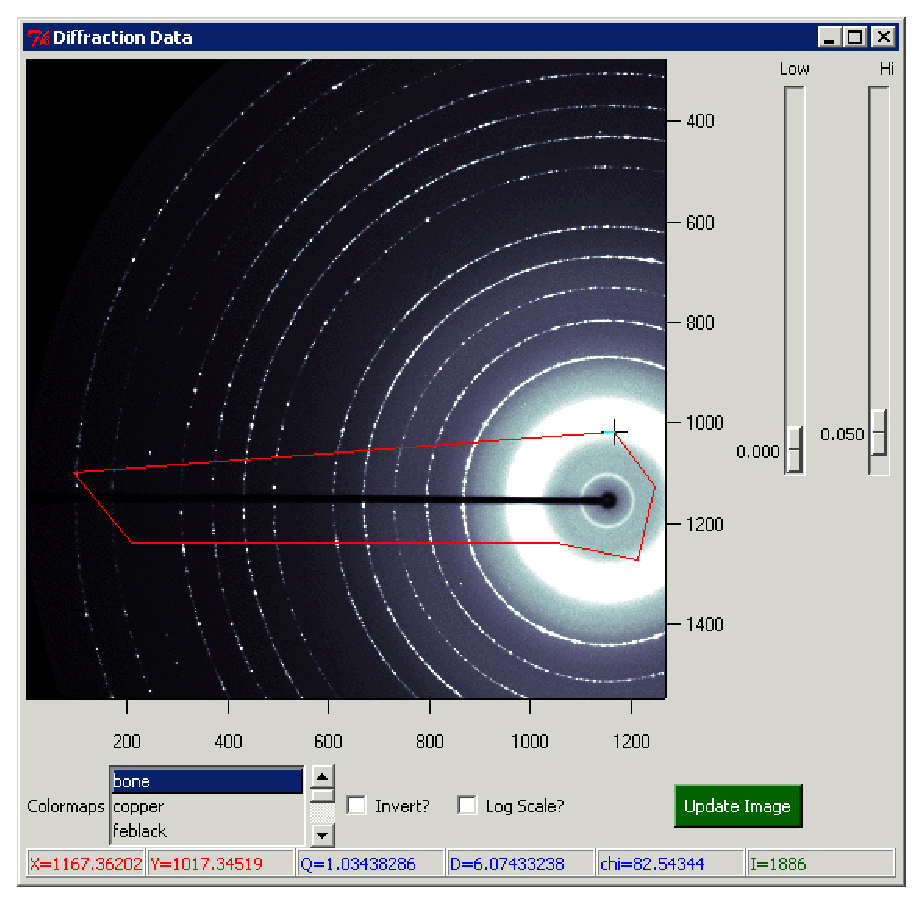
\includegraphics[scale=.75]{figures/Adding_Polygon.eps}
    \caption{A new polygon mask is being added to the 
    program. This particular mask will cover 
    the beam stop.}
    \label{Adding_Polygon}
\end{SCfigure}

A polygon mask can be added to the image with
the \gui{Add Polygon} button on the \gui{Masking} tab. 
This button will stay down when pushed and puts
the program in polygon drawing mode.  In this mode, the 
diffraction image can no longer be zoomed or panned.
Instead, left clicking on the diffraction image will make
the program draw a polygon mask.  The first left click adds the
first vertex. Each success left click add another vertex. 
The drawing can be finished and the final vertex added by right 
clicking. The program return to its
normal state and add the polygon into the program. 
Multiple polygons can be added using the \gui{Add Polygon}
button. Figure~\ref{Adding_Polygon} shows 
the program when a polygon is
being drawn. A half drawn polygon can be aborted without finishing
it by unpushing the \gui{Add Polygon} button.

\begin{SCfigure}[1][bthp]
    \centering
    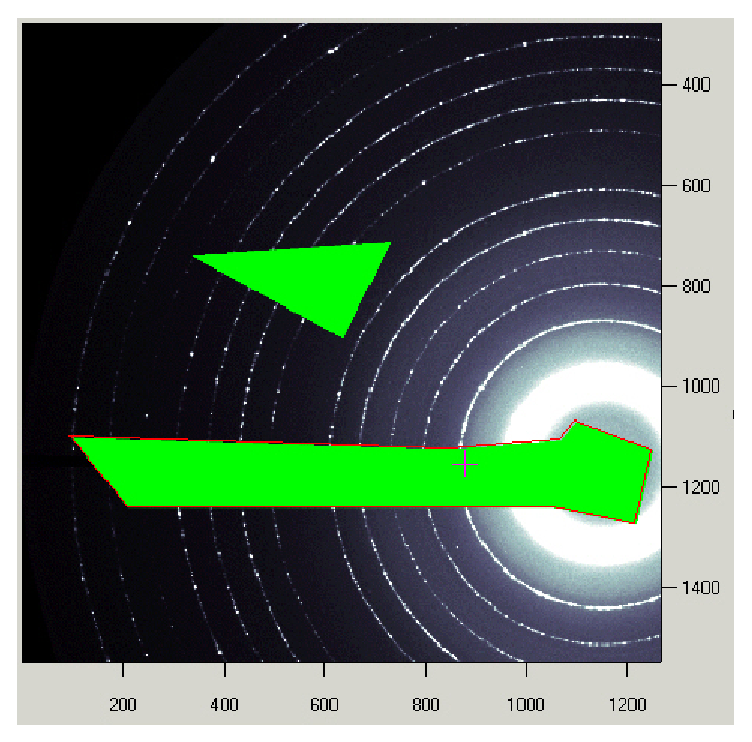
\includegraphics[scale=.75]{figures/Removing_Polygon.eps}
    \caption{A polygon is about to be removed.
    When mousing over a polygon to remove it,
    the program will display a red border around it.}
    \label{Removing_Polygon}
\end{SCfigure}

The \gui{Remove Polygon} button can be used to remove
a polygon from the program. Like the \gui{Add Polygon} 
button, this button will stay pushed and change the
behavior of the diffraction image. After pushing the 
\gui{Remove Polygon} button, clicking over
a particular polygon will remove it.
After the polygon is removed, the program will 
return to its normal state.
Figure~\ref{Removing_Polygon} shows what the diffraction
window looks like when a polygon is about to be removed.
The program can return to its normal state without
removing a polygon by unpushing the \gui{Remove Polgyon}
button.

The \gui{Clear Mask} button can be used to remove
all the polygons at once. The \gui{Save Mask} button
can be used to save all the polygons to a file.
A file of polygons can be added to the program 
using the 
\gui{Load Mask} button. A polygon
file is very simple. The polygons in 
figure~\ref{Displayed_Polygon} were saved as
\begin{lstlisting}[caption={'polygons.dat'}]
# Polygon(s) drawn on Thu Feb 07 00:00:21 2008
93.140587183	1098.06704199
208.013978042	1237.77792276
1052.48863517	1237.77792276
1213.93231962	1271.92947139
1248.08386825	1126.00921814
1095.95424252	1067.02017959
1064.90738013	1104.27641447
847.579343365	1122.9045319

332.201427619	737.923438212
633.355992844	902.471808902
729.601266267	709.981262058
\end{lstlisting}
Each line is an ($x$,$y$) coordinate for one of 
the nodes of the polygon.  The coordinates are separated
by spaces. Each polygon is separated by a newline.  
Comment lines beginning with \# are 
ignored. 

\section{Masking Caked Plots}

Any polygon masks or threshold masks will also 
show up on the caked plot. As figure~\ref{box_mask} shows, 
polygons on a diffraction image can look very distorted on 
a caked plot. 

\begin{figure}[htb]
    \centering
    \subfloat[A rectangular polygon mask in 
    the middle of a diffraction image]{
    \label{box_mask_diffraction}
    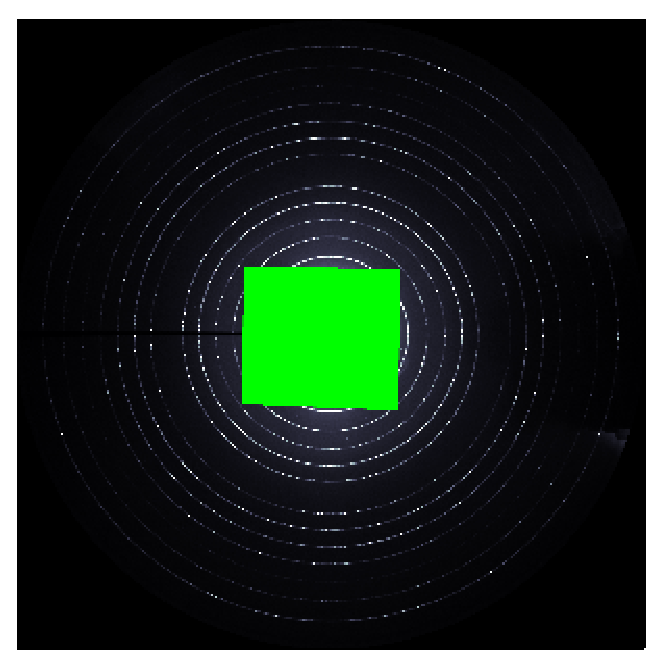
\includegraphics[scale=.7]
    {figures/box_mask_diffraction_image.eps}}\hspace{1em}
    \subfloat[The same rectangular mask on
    a caked plot]{
    \label{box_mask_cake}
    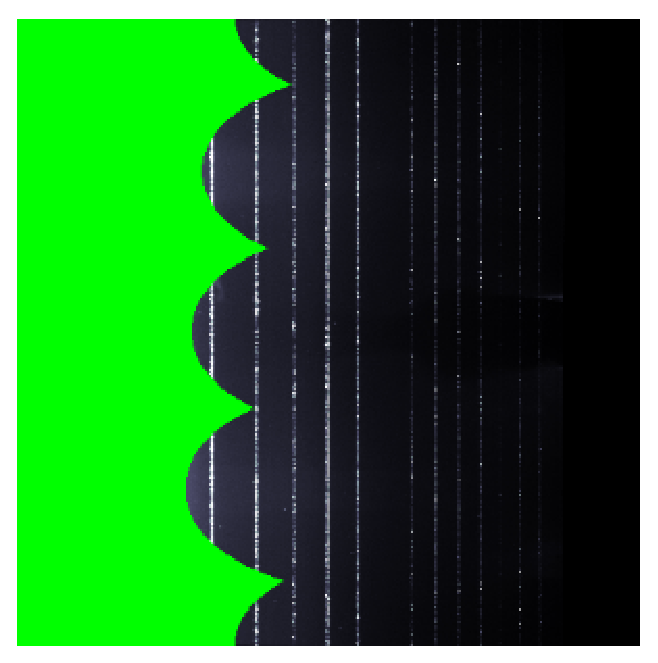
\includegraphics[scale=.7]{figures/box_mask_cake_image.eps}}
    \caption{A relatively simple shape on a diffraction image 
    can look very different on a caked plot.}
    \label{box_mask}
\end{figure}



